\section{Generate Test Cases}

Lacking test cases of known properties is one common problem in
developing software for machine learning.  The purpose of machine
learning is to recognize unknown patterns in data.  How can we know
that the programs are correct if we do not know what the programs
should find?
Two methods are commonly used:
\begin{enumerate}
\item Creating simple test cases manually with known patterns.

\item Adopting widely used test cases whose patterns have already
  been studied.
\end{enumerate}
The first methods is restricted to only very small test cases that are
unlikely to have sophisticated patterns needed to test computer
programs.  The second methods, in contrast, may have sophisticated
patterns but the data may be too complex for identifying problems in
the programs.

\index{test case generator}


This book suggests the third approach: write another program (or
several programs, called {\it test case generators}) to generate the
test cases of known patterns.  More specifically, for this problem, we
can write a program that generates $n$ data points in $k$ clusters ($n
> k$).  Since the data points are generated intentionally, it is easy
to test whether a k-mean program is correct.


Writing a test case generator, however, is not trivial because the
generator has to consider many different possible properties of data
collected in different scenarios. It is likely that different
generators would be needed in different scenarios. This section
explains one generator. Readers may need to change this generator to
meet different needs.  The programs in this chapter handles integers
only because floating-point numbers have limited precision and
sometimes give surprising results, to be discussed later in this book.
This program generates two output files: {\tt data.txt} and {\tt
  cluster.txt}.  The first file has $n$ lines and each line has $p$
integers.  The second file also has $n$ lines; each line has the same
$p$ integers, following by one integer between $0$ and $m - 1$ to
indicate which cluster this line belongs to.

\resetlinenumber[1]
\linenumbers
\begin{tt}
  \lstinputlisting{\progpath/unsupervised/kmean/testgen/main.py}
\end{tt}
\nolinenumbers

This is {\tt testgen.py}.

\resetlinenumber[1]
\linenumbers
\begin{tt}
  \lstinputlisting{\progpath/unsupervised/kmean/testgen/testgen.py}
\end{tt}
\nolinenumbers


To run the program using the default values, type {\tt python3
  main.py}.  This is an example output {\tt data.txt}:

\begin{tt}
  \lstinputlisting{\kmeanpath/data/data1.txt}
\end{tt}

This is an example of the corresponding {\tt cluster.txt}.

\begin{tt}
  \lstinputlisting{\kmeanpath/data/cluster1.txt}
\end{tt}

\section{Visualize Data}

\index{high-dimensional}

This program can visualize data up to three dimensions.  The purpose
of this visualization is to help inspect whether the data produced by
the test generator is indeed clustered into several regions.

\resetlinenumber[1]
\linenumbers
\begin{tt}
  \lstinputlisting{\progpath/unsupervised/kmean/testgen/visualize.py}
\end{tt}
\nolinenumbers

The following figure visualizes the generated data
shown earlier.

\begin{figure}[h] \centering
{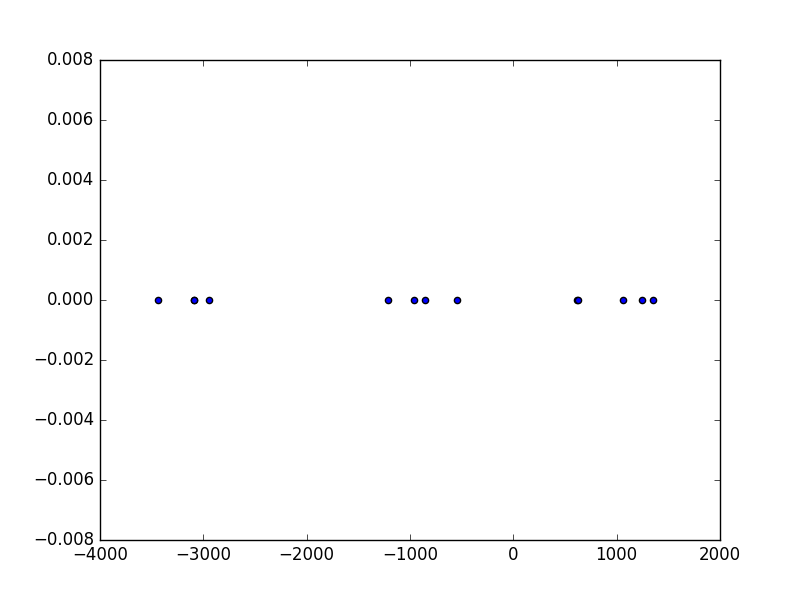
\includegraphics[width=3in]{\kmeanpath/figures/figure1.png}}
\caption{Visualize the generated test case. }
\end{figure}


The figures show more examples.

\begin{figure}[h] \centering
 \subfigure[]
{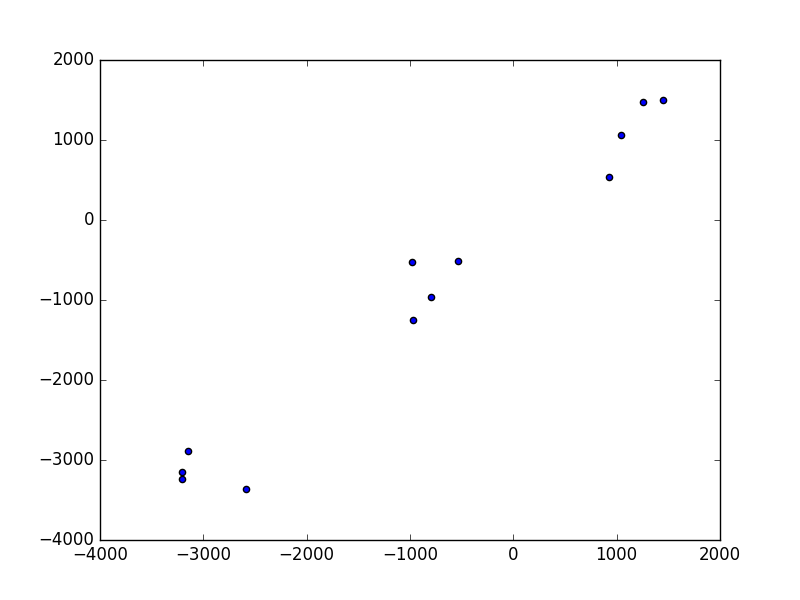
\includegraphics[width=3in]{\kmeanpath/figures/figure2.png}}
  \subfigure[]
{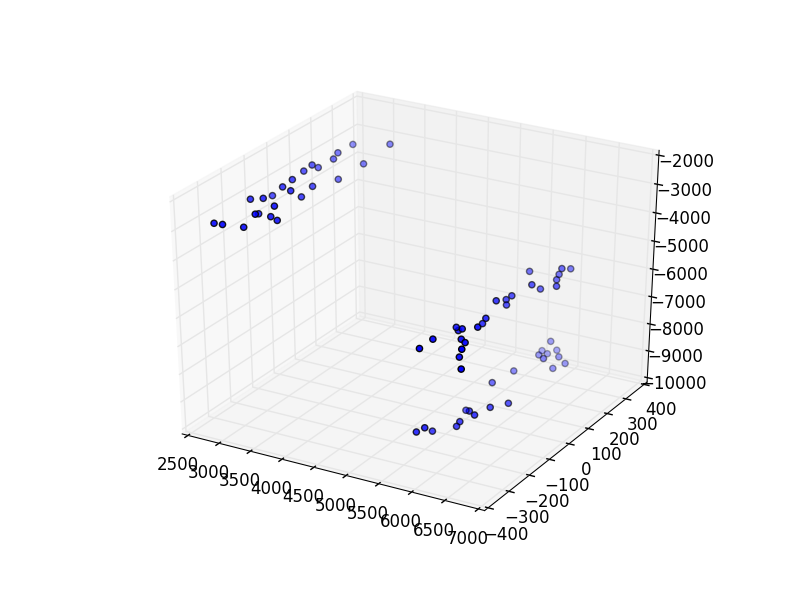
\includegraphics[width=3in]{\kmeanpath/figures/figure3.png}}
  \subfigure[]
{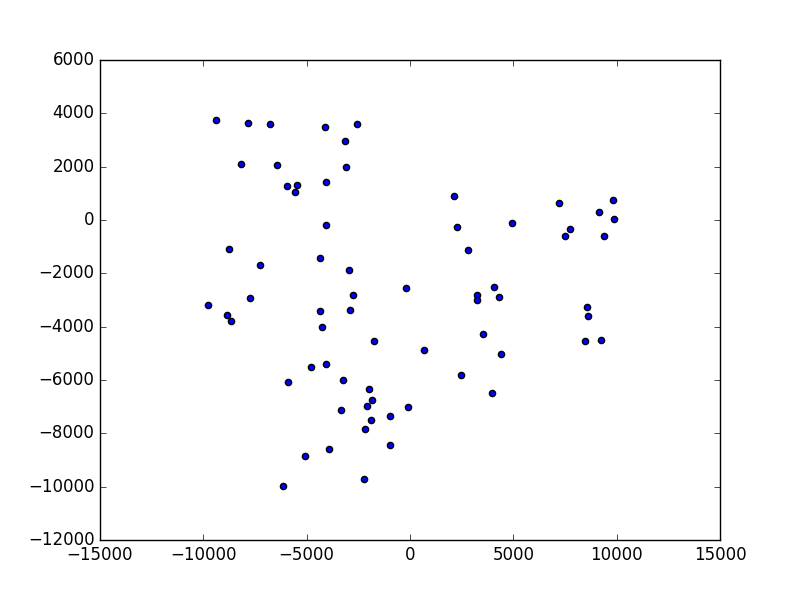
\includegraphics[width=3in]{\kmeanpath/figures/figure4.png}}
\caption{Visualize the generated test cases with different arguments:
  (a) {\tt python3 main.py -d 1 -m 4}, (b) {\tt python3 main.py -d 3 -m
    3}, (c) {\tt python3 main.py -t -m 3}. }
\end{figure}

\clearpage

\section{K-Mean Algorithm Implementation}

Now is the time to show how the {\it K-Mean} algorithm can be
implemented. The implementation pretty much reflects the algorithm
described on Page~\pageref{algorithm:kmean}.

\resetlinenumber[1]
\linenumbers
\begin{tt}
  \lstinputlisting{\progpath/unsupervised/kmean/solution/main.py}
\end{tt}
\nolinenumbers

\resetlinenumber[1]
\linenumbers
\begin{tt}
  \lstinputlisting{\progpath/unsupervised/kmean/solution/kmean.py}
\end{tt}
\nolinenumbers

\resetlinenumber[1]
\linenumbers
\begin{tt}
  \lstinputlisting{\progpath/unsupervised/kmean/solution/datapoint.py}
\end{tt}
\nolinenumbers

\resetlinenumber[1]
\linenumbers
\begin{tt}
  \lstinputlisting{\progpath/unsupervised/kmean/solution/centroid.py}
\end{tt}
\nolinenumbers


Does this program work? Let's try an example.
Figure~\ref{figure:kmean:56} (a) clearly shows three clusters
and Figure~\ref{figure:kmean:56} (b) shows the clusters have been
marked by different labels. The result is pretty encouraging.

\begin{figure}[h] \centering
 \subfigure[]
{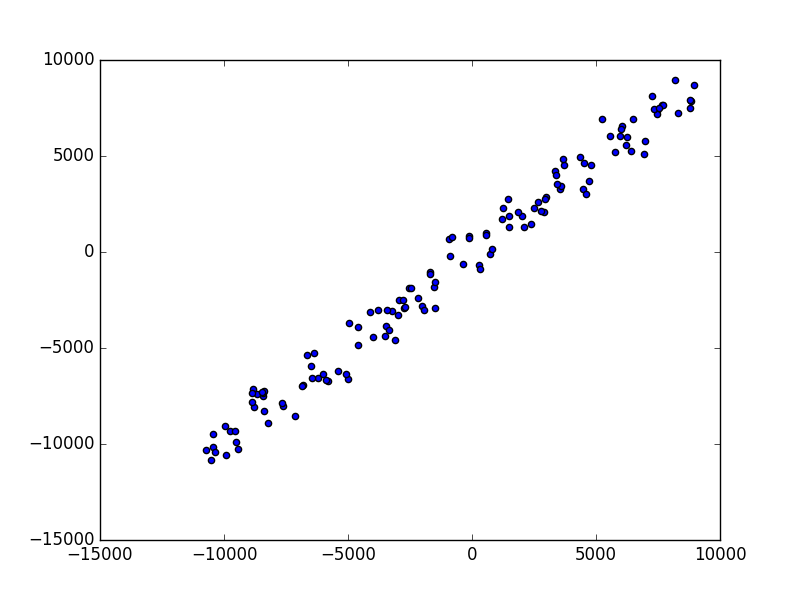
\includegraphics[width=3in]{\kmeanpath/figures/figure5.png}}
  \subfigure[]
{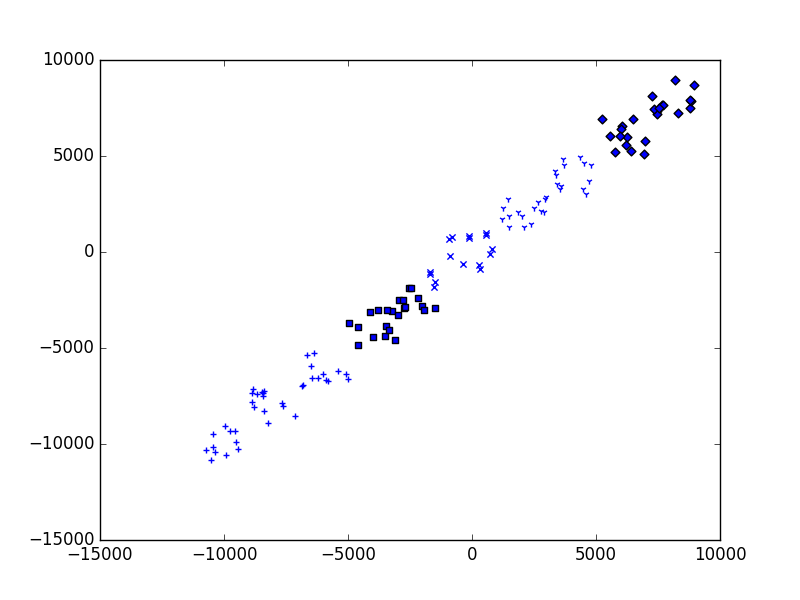
\includegraphics[width=3in]{\kmeanpath/figures/figure6.png}}
\caption{Visualize the generated by (a) 
  (a) {\tt python3 main.py}, (b) Result of running {\tt python3 main.py data.txt 3}. }
\label{figure:kmean:56}
\end{figure}




\clearpage
Figure~\ref{figure:kmean:56} (b) is generated by using different
symbols for the clusters. It is a slightly different visualization
program:

\resetlinenumber[1]
\linenumbers
\begin{tt}
  \lstinputlisting{\progpath/unsupervised/kmean/solution/visualize.py}
\end{tt}
\nolinenumbers

\clearpage
So far the data is generated by the test case generator and the data
points are clearly clustered without any overlap.  Now, let's consider
some variations.

\begin{figure}[h] \centering
  \subfigure[]
  {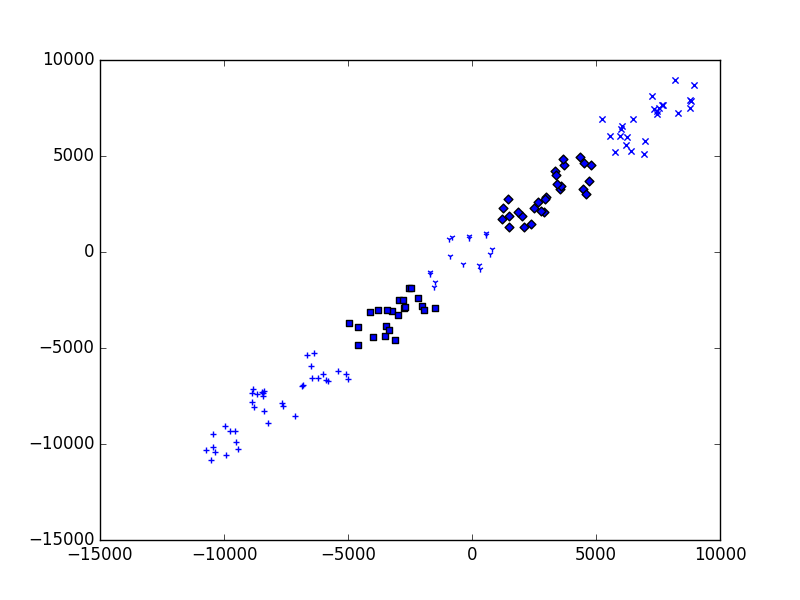
\includegraphics[width=4in]{\kmeanpath/figures/figure7.png}}
  \subfigure[]
{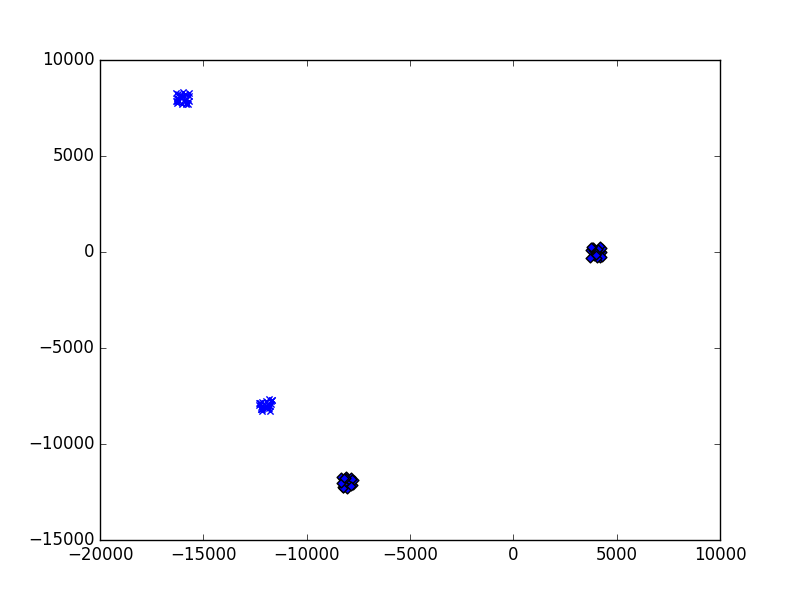
\includegraphics[width=4in]{\kmeanpath/figures/figure8.png}}
\caption{(a) Data generated using {\tt  python3 main.py -m 4}.
(b) K-Mean result using 2 clusters (i.e., $k$ is 2). }
\end{figure}

\clearpage

The next example allows clusters to overlap by adding {\tt -t} in
the test generator.

\begin{figure}[h] \centering
  \subfigure[]
  {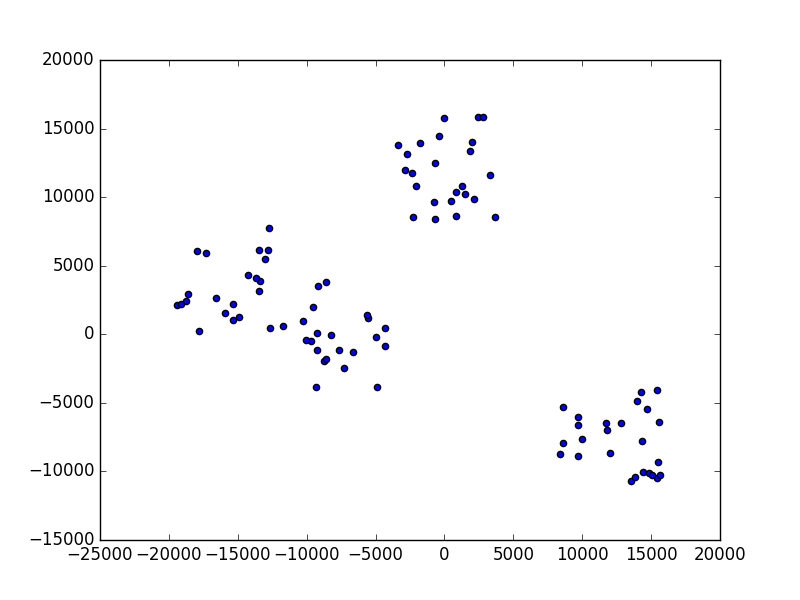
\includegraphics[width=4in]{\kmeanpath/figures/figure9.png}}
  \subfigure[]
{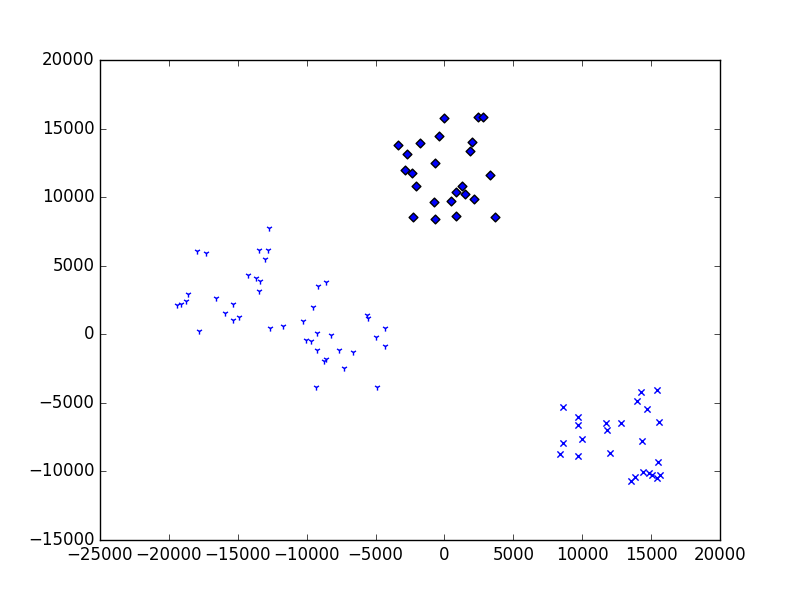
\includegraphics[width=4in]{\kmeanpath/figures/figure10.png}}
\caption{(a) Data generated using {\tt  python3 main.py -t -m 4}.
(b) K-Mean result using 3 clusters. }
\end{figure}

\clearpage

\section{Understand Non-Deterministic Behavior of K-Mean}

This is great, right? Let us run the clustering program using 4 clusters
twice:

\begin{figure}[h] \centering
  \subfigure[]
  {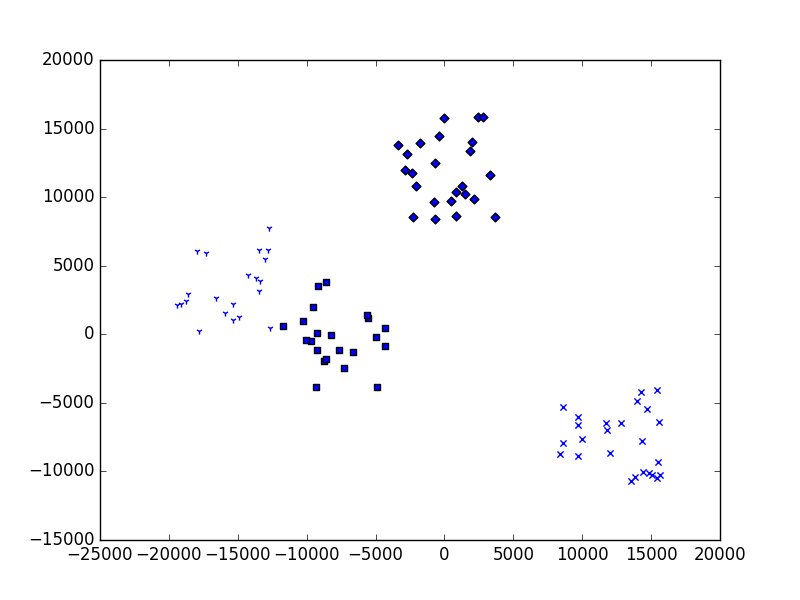
\includegraphics[width=3in]{\kmeanpath/figures/figure11.png}}
  \subfigure[]
  {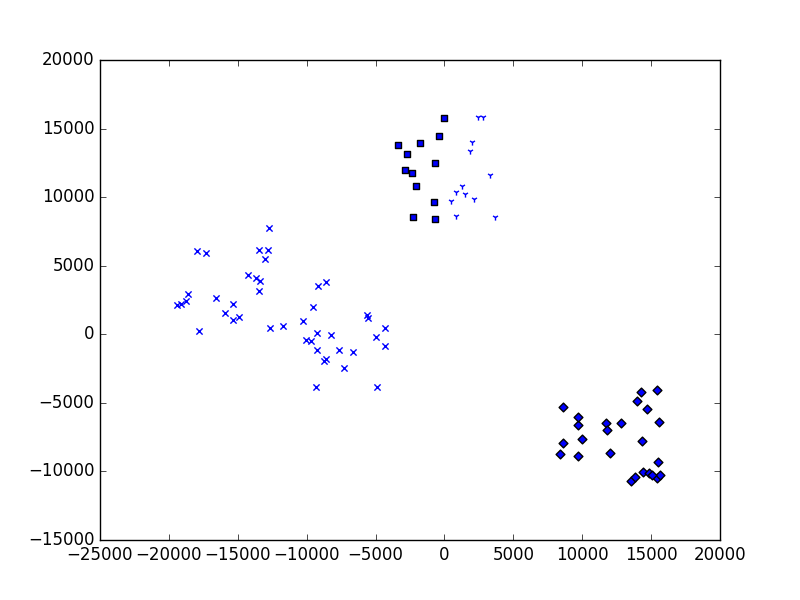
\includegraphics[width=3in]{\kmeanpath/figures/figure12.png}}
  \subfigure[]
{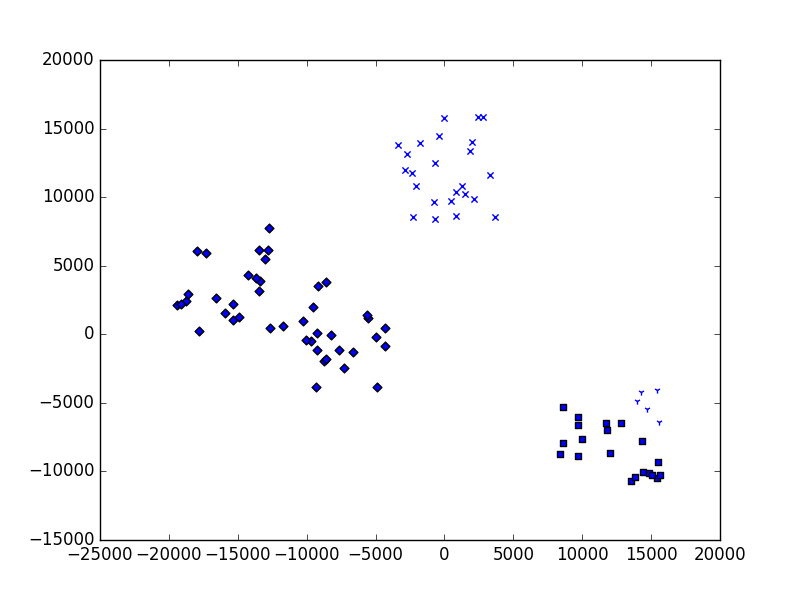
\includegraphics[width=3in]{\kmeanpath/figures/figure13.png}}
\caption{Running the k-mean program three times using 4 clusters. }
\label{figure:kmean:1112}
\end{figure}

\clearpage

Figure~\ref{figure:kmean:1112} (a) seems pretty reasonable
but Figure~\ref{figure:kmean:1112} (b) and (c) do not look right.
How can this program produces different
results even though the input data is the same?  A simple
answer is that this program is {\it non-deterministic}.
The reason this program is non-deterministic is this line in
{\tt kmean.py}:

\index{non-deterministic}
\begin{verbatim}
        clu = random.randint(0, kval - 1)
\end{verbatim}

\index{random number generator}

It assigns each data point to a cluster between $0$ and $k-1$
randomly.  It is possible that two or more data points in the same
cluster (by the test generator) are assigned to different clusters.

Python (and most programming languages) has a {\it random number
  generator}.  It generates random numbers. What does this mean?  It
means that it would be difficult to predict the next number after
observing a sequence of numbers.  Let us consider several
examples. This is a simply program calling Python's {\tt
  random.randint}.

\resetlinenumber[1]
\linenumbers
\begin{tt}
  \lstinputlisting{\progpath/unsupervised/kmean/random/sequence1.py}
\end{tt}
\nolinenumbers

The following shows the results
executing the program three times; each column is the result of
executing the program once.

\begin{tabular}{p{1in}p{1in}p{1in}}
\begin{tt}
  \lstinputlisting{\kmeanpath/data/sequence1.txt}
\end{tt}
&
\begin{tt}
  \lstinputlisting{\kmeanpath/data/sequence2.txt}
\end{tt}

&
\begin{tt}
  \lstinputlisting{\kmeanpath/data/sequence3.txt}
\end{tt}

\end{tabular}

Reading top to bottom inside each column, it is difficult to predict
the next number from the numbers that have already been seen.
Comparing different columns, the sequences are different.

\index{random number generator!seed}
Python allows programmers to set  the {\it seed} of the random number generator.
If the same seed is same, the same sequence of numbers is generated.
In other words, the sequence becomes {\it deterministic}.  The following program
always generates the same sequence of numbers.


\resetlinenumber[1]
\linenumbers
\begin{tt}
  \lstinputlisting{\progpath/unsupervised/kmean/random/sequence2.py}
\end{tt}
\nolinenumbers

\index{security key}

The words {\it random} and {\it non-deterministic} are often confused.
Random means it is difficult to predict in advance.  {\it
  Non-deterministic} means that if the same program runs again with
the same inputs, the results may be different.  It is possible to have
a deterministic sequence of random numbers, like the ones generated by
{\tt sequence2.py}.  The sequence is deterministic because running the
program again generates the same sequence. The sequence is random
because knowing the generated numbers cannot predict the future
numbers.

\index{random number generator!seed}


A common way of varying the seed is using the microsecond of the
current time in the following way:

\begin{verbatim}
        random.seed(datetime.datetime.now().microsecond)
\end{verbatim}

Be careful using time as random number seeds for keys in security
programs.  Using microseconds restrict the possible keys to only 0 and
999999.  This small range of seeds weakens security because there are
only one million possibilities.

